%%%%%%%%%%%%%%%%%%%%%%%%%%%%%%%%%%%%%%%%%
% The Legrand Orange Book
% LaTeX Template
% Version 2.1.1 (14/2/16)
%
% This template has been downloaded from:
% http://www.LaTeXTemplates.com
%
% Original author:
% Mathias Legrand (legrand.mathias@gmail.com) with modifications by:
% Vel (vel@latextemplates.com)
%
% License:
% CC BY-NC-SA 3.0 (http://creativecommons.org/licenses/by-nc-sa/3.0/)
%
% Compiling this template:
% This template uses biber for its bibliography and makeindex for its index.
% When you first open the template, compile it from the command line with the
% commands below to make sure your LaTeX distribution is configured correctly:
%
% 1) pdflatex main
% 2) makeindex main.idx -s StyleInd.ist
% 3) biber main
% 4) pdflatex main x 2
%
% After this, when you wish to update the bibliography/index use the appropriate
% command above and make sure to compile with pdflatex several times
% afterwards to propagate your changes to the document.
%
% This template also uses a number of packages which may need to be
% updated to the newest versions for the template to compile. It is strongly
% recommended you update your LaTeX distribution if you have any
% compilation errors.
%
% Important note:
% Chapter heading images should have a 2:1 width:height ratio,
% e.g. 920px width and 460px height.
%
%%%%%%%%%%%%%%%%%%%%%%%%%%%%%%%%%%%%%%%%%

%----------------------------------------------------------------------------------------
%	PACKAGES AND OTHER DOCUMENT CONFIGURATIONS
%----------------------------------------------------------------------------------------

\documentclass[11pt,fleqn]{book} % Default font size and left-justified equations

%----------------------------------------------------------------------------------------

%%%%%%%%%%%%%%%%%%%%%%%%%%%%%%%%%%%%%%%%%
% The Legrand Orange Book
% Structural Definitions File
% Version 2.0 (9/2/15)
%
% Original author:
% Mathias Legrand (legrand.mathias@gmail.com) with modifications by:
% Vel (vel@latextemplates.com)
%
% This file has been downloaded from:
% http://www.LaTeXTemplates.com
%
% License:
% CC BY-NC-SA 3.0 (http://creativecommons.org/licenses/by-nc-sa/3.0/)
%
%%%%%%%%%%%%%%%%%%%%%%%%%%%%%%%%%%%%%%%%%

%----------------------------------------------------------------------------------------
%	VARIOUS REQUIRED PACKAGES AND CONFIGURATIONS
%----------------------------------------------------------------------------------------

\usepackage[top=3cm,bottom=3cm,left=3cm,right=3cm,headsep=10pt,a4paper]{geometry} % Page margins

\usepackage{kotex}
\usepackage{graphicx} % Required for including pictures
\graphicspath{{Pictures/}} % Specifies the directory where pictures are stored

\usepackage{lipsum} % Inserts dummy text

\usepackage{tikz} % Required for drawing custom shapes

\usepackage[english]{babel} % English language/hyphenation

\usepackage{enumitem} % Customize lists
\setlist{nolistsep} % Reduce spacing between bullet points and numbered lists

\usepackage{booktabs} % Required for nicer horizontal rules in tables

\usepackage{xcolor} % Required for specifying colors by name
\definecolor{ocre}{RGB}{243,102,25} % Define the orange color used for highlighting throughout the book

%----------------------------------------------------------------------------------------
%	FONTS
%----------------------------------------------------------------------------------------

\usepackage{avant} % Use the Avantgarde font for headings
%\usepackage{times} % Use the Times font for headings
\usepackage{mathptmx} % Use the Adobe Times Roman as the default text font together with math symbols from the Sym­bol, Chancery and Com­puter Modern fonts

\usepackage{microtype} % Slightly tweak font spacing for aesthetics
\usepackage[utf8]{inputenc} % Required for including letters with accents
\usepackage[T1]{fontenc} % Use 8-bit encoding that has 256 glyphs

%----------------------------------------------------------------------------------------
%	BIBLIOGRAPHY AND INDEX
%----------------------------------------------------------------------------------------

\usepackage[style=alphabetic,citestyle=numeric,sorting=nyt,sortcites=true,autopunct=true,babel=hyphen,hyperref=true,abbreviate=false,backref=true,backend=biber]{biblatex}
\addbibresource{bibliography.bib} % BibTeX bibliography file
\defbibheading{bibempty}{}

\usepackage{calc} % For simpler calculation - used for spacing the index letter headings correctly
\usepackage{makeidx} % Required to make an index
\makeindex % Tells LaTeX to create the files required for indexing

%----------------------------------------------------------------------------------------
%	MAIN TABLE OF CONTENTS
%----------------------------------------------------------------------------------------

\usepackage{titletoc} % Required for manipulating the table of contents

\contentsmargin{0cm} % Removes the default margin

% Part text styling
\titlecontents{part}[0cm]
{\addvspace{20pt}\centering\large\bfseries}
{}
{}
{}

% Chapter text styling
\titlecontents{chapter}[1.25cm] % Indentation
{\addvspace{12pt}\large\sffamily\bfseries} % Spacing and font options for chapters
{\color{ocre!60}\contentslabel[\Large\thecontentslabel]{1.25cm}\color{ocre}} % Chapter number
{\color{ocre}}
{\color{ocre!60}\normalsize\;\titlerule*[.5pc]{.}\;\thecontentspage} % Page number

% Section text styling
\titlecontents{section}[1.25cm] % Indentation
{\addvspace{3pt}\sffamily\bfseries} % Spacing and font options for sections
{\contentslabel[\thecontentslabel]{1.25cm}} % Section number
{}
{\hfill\color{black}\thecontentspage} % Page number
[]

% Subsection text styling
\titlecontents{subsection}[1.25cm] % Indentation
{\addvspace{1pt}\sffamily\small} % Spacing and font options for subsections
{\contentslabel[\thecontentslabel]{1.25cm}} % Subsection number
{}
{\ \titlerule*[.5pc]{.}\;\thecontentspage} % Page number
[]

% List of figures
\titlecontents{figure}[0em]
{\addvspace{-5pt}\sffamily}
{\thecontentslabel\hspace*{1em}}
{}
{\ \titlerule*[.5pc]{.}\;\thecontentspage}
[]

% List of tables
\titlecontents{table}[0em]
{\addvspace{-5pt}\sffamily}
{\thecontentslabel\hspace*{1em}}
{}
{\ \titlerule*[.5pc]{.}\;\thecontentspage}
[]

%----------------------------------------------------------------------------------------
%	MINI TABLE OF CONTENTS IN PART HEADS
%----------------------------------------------------------------------------------------

% Chapter text styling
\titlecontents{lchapter}[0em] % Indenting
{\addvspace{15pt}\large\sffamily\bfseries} % Spacing and font options for chapters
{\color{ocre}\contentslabel[\Large\thecontentslabel]{1.25cm}\color{ocre}} % Chapter number
{}
{\color{ocre}\normalsize\sffamily\bfseries\;\titlerule*[.5pc]{.}\;\thecontentspage} % Page number

% Section text styling
\titlecontents{lsection}[0em] % Indenting
{\sffamily\small} % Spacing and font options for sections
{\contentslabel[\thecontentslabel]{1.25cm}} % Section number
{}
{}

% Subsection text styling
\titlecontents{lsubsection}[.5em] % Indentation
{\normalfont\footnotesize\sffamily} % Font settings
{}
{}
{}

%----------------------------------------------------------------------------------------
%	PAGE HEADERS
%----------------------------------------------------------------------------------------

\usepackage{fancyhdr} % Required for header and footer configuration

\pagestyle{fancy}
\renewcommand{\chaptermark}[1]{\markboth{\sffamily\normalsize\bfseries\chaptername\ \thechapter.\ #1}{}} % Chapter text font settings
\renewcommand{\sectionmark}[1]{\markright{\sffamily\normalsize\thesection\hspace{5pt}#1}{}} % Section text font settings
\fancyhf{} \fancyhead[LE,RO]{\sffamily\normalsize\thepage} % Font setting for the page number in the header
\fancyhead[LO]{\rightmark} % Print the nearest section name on the left side of odd pages
\fancyhead[RE]{\leftmark} % Print the current chapter name on the right side of even pages
\renewcommand{\headrulewidth}{0.5pt} % Width of the rule under the header
\addtolength{\headheight}{2.5pt} % Increase the spacing around the header slightly
\renewcommand{\footrulewidth}{0pt} % Removes the rule in the footer
\fancypagestyle{plain}{\fancyhead{}\renewcommand{\headrulewidth}{0pt}} % Style for when a plain pagestyle is specified

% Removes the header from odd empty pages at the end of chapters
\makeatletter
\renewcommand{\cleardoublepage}{
\clearpage\ifodd\c@page\else
\hbox{}
\vspace*{\fill}
\thispagestyle{empty}
\newpage
\fi}

%----------------------------------------------------------------------------------------
%	THEOREM STYLES
%----------------------------------------------------------------------------------------

\usepackage{amsmath,amsfonts,amssymb,amsthm} % For math equations, theorems, symbols, etc

\newcommand{\intoo}[2]{\mathopen{]}#1\,;#2\mathclose{[}}
\newcommand{\ud}{\mathop{\mathrm{{}d}}\mathopen{}}
\newcommand{\intff}[2]{\mathopen{[}#1\,;#2\mathclose{]}}
\newtheorem{notation}{Notation}[chapter]

% Boxed/framed environments
\newtheoremstyle{ocrenumbox}% % Theorem style name
{0pt}% Space above
{0pt}% Space below
{\normalfont}% % Body font
{}% Indent amount
{\small\bf\sffamily\color{ocre}}% % Theorem head font
{\;}% Punctuation after theorem head
{0.25em}% Space after theorem head
{\small\sffamily\color{ocre}\thmname{#1}\nobreakspace\thmnumber{\@ifnotempty{#1}{}\@upn{#2}}% Theorem text (e.g. Theorem 2.1)
\thmnote{\nobreakspace\the\thm@notefont\sffamily\bfseries\color{black}---\nobreakspace#3.}} % Optional theorem note
\renewcommand{\qedsymbol}{$\blacksquare$}% Optional qed square

\newtheoremstyle{blacknumex}% Theorem style name
{5pt}% Space above
{5pt}% Space below
{\normalfont}% Body font
{} % Indent amount
{\small\bf\sffamily}% Theorem head font
{\;}% Punctuation after theorem head
{0.25em}% Space after theorem head
{\small\sffamily{\tiny\ensuremath{\blacksquare}}\nobreakspace\thmname{#1}\nobreakspace\thmnumber{\@ifnotempty{#1}{}\@upn{#2}}% Theorem text (e.g. Theorem 2.1)
\thmnote{\nobreakspace\the\thm@notefont\sffamily\bfseries---\nobreakspace#3.}}% Optional theorem note

\newtheoremstyle{blacknumbox} % Theorem style name
{0pt}% Space above
{0pt}% Space below
{\normalfont}% Body font
{}% Indent amount
{\small\bf\sffamily}% Theorem head font
{\;}% Punctuation after theorem head
{0.25em}% Space after theorem head
{\small\sffamily\thmname{#1}\nobreakspace\thmnumber{\@ifnotempty{#1}{}\@upn{#2}}% Theorem text (e.g. Theorem 2.1)
\thmnote{\nobreakspace\the\thm@notefont\sffamily\bfseries---\nobreakspace#3.}}% Optional theorem note

% Non-boxed/non-framed environments
\newtheoremstyle{ocrenum}% % Theorem style name
{5pt}% Space above
{5pt}% Space below
{\normalfont}% % Body font
{}% Indent amount
{\small\bf\sffamily\color{ocre}}% % Theorem head font
{\;}% Punctuation after theorem head
{0.25em}% Space after theorem head
{\small\sffamily\color{ocre}\thmname{#1}\nobreakspace\thmnumber{\@ifnotempty{#1}{}\@upn{#2}}% Theorem text (e.g. Theorem 2.1)
\thmnote{\nobreakspace\the\thm@notefont\sffamily\bfseries\color{black}---\nobreakspace#3.}} % Optional theorem note
\renewcommand{\qedsymbol}{$\blacksquare$}% Optional qed square
\makeatother

% Defines the theorem text style for each type of theorem to one of the three styles above
\newcounter{dummy}
\numberwithin{dummy}{section}
\theoremstyle{ocrenumbox}
\newtheorem{theoremeT}[dummy]{Theorem}
\newtheorem{problem}{Problem}[chapter]
\newtheorem{exerciseT}{Exercise}[chapter]
\theoremstyle{blacknumex}
\newtheorem{exampleT}{Example}[chapter]
\theoremstyle{blacknumbox}
\newtheorem{vocabulary}{Vocabulary}[chapter]
\newtheorem{definitionT}{Definition}[section]
\newtheorem{corollaryT}[dummy]{Corollary}
\theoremstyle{ocrenum}
\newtheorem{proposition}[dummy]{Proposition}

%----------------------------------------------------------------------------------------
%	DEFINITION OF COLORED BOXES
%----------------------------------------------------------------------------------------

\RequirePackage[framemethod=default]{mdframed} % Required for creating the theorem, definition, exercise and corollary boxes

% Theorem box
\newmdenv[skipabove=7pt,
skipbelow=7pt,
backgroundcolor=black!5,
linecolor=ocre,
innerleftmargin=5pt,
innerrightmargin=5pt,
innertopmargin=5pt,
leftmargin=0cm,
rightmargin=0cm,
innerbottommargin=5pt]{tBox}

% Exercise box
\newmdenv[skipabove=7pt,
skipbelow=7pt,
rightline=false,
leftline=true,
topline=false,
bottomline=false,
backgroundcolor=ocre!10,
linecolor=ocre,
innerleftmargin=5pt,
innerrightmargin=5pt,
innertopmargin=5pt,
innerbottommargin=5pt,
leftmargin=0cm,
rightmargin=0cm,
linewidth=4pt]{eBox}

% Definition box
\newmdenv[skipabove=7pt,
skipbelow=7pt,
rightline=false,
leftline=true,
topline=false,
bottomline=false,
linecolor=ocre,
innerleftmargin=5pt,
innerrightmargin=5pt,
innertopmargin=0pt,
leftmargin=0cm,
rightmargin=0cm,
linewidth=4pt,
innerbottommargin=0pt]{dBox}

% Corollary box
\newmdenv[skipabove=7pt,
skipbelow=7pt,
rightline=false,
leftline=true,
topline=false,
bottomline=false,
linecolor=gray,
backgroundcolor=black!5,
innerleftmargin=5pt,
innerrightmargin=5pt,
innertopmargin=5pt,
leftmargin=0cm,
rightmargin=0cm,
linewidth=4pt,
innerbottommargin=5pt]{cBox}

% Creates an environment for each type of theorem and assigns it a theorem text style from the "Theorem Styles" section above and a colored box from above
\newenvironment{theorem}{\begin{tBox}\begin{theoremeT}}{\end{theoremeT}\end{tBox}}
\newenvironment{exercise}{\begin{eBox}\begin{exerciseT}}{\hfill{\color{ocre}\tiny\ensuremath{\blacksquare}}\end{exerciseT}\end{eBox}}
\newenvironment{definition}{\begin{dBox}\begin{definitionT}}{\end{definitionT}\end{dBox}}
\newenvironment{example}{\begin{exampleT}}{\hfill{\tiny\ensuremath{\blacksquare}}\end{exampleT}}
\newenvironment{corollary}{\begin{cBox}\begin{corollaryT}}{\end{corollaryT}\end{cBox}}

%----------------------------------------------------------------------------------------
%	REMARK ENVIRONMENT
%----------------------------------------------------------------------------------------

\newenvironment{remark}{\par\vspace{10pt}\small % Vertical white space above the remark and smaller font size
\begin{list}{}{
\leftmargin=35pt % Indentation on the left
\rightmargin=25pt}\item\ignorespaces % Indentation on the right
\makebox[-2.5pt]{\begin{tikzpicture}[overlay]
\node[draw=ocre!60,line width=1pt,circle,fill=ocre!25,font=\sffamily\bfseries,inner sep=2pt,outer sep=0pt] at (-15pt,0pt){\textcolor{ocre}{R}};\end{tikzpicture}} % Orange R in a circle
\advance\baselineskip -1pt}{\end{list}\vskip5pt} % Tighter line spacing and white space after remark

%----------------------------------------------------------------------------------------
%	SECTION NUMBERING IN THE MARGIN
%----------------------------------------------------------------------------------------

\makeatletter
\renewcommand{\@seccntformat}[1]{\llap{\textcolor{ocre}{\csname the#1\endcsname}\hspace{1em}}}
\renewcommand{\section}{\@startsection{section}{1}{\z@}
{-4ex \@plus -1ex \@minus -.4ex}
{1ex \@plus.2ex }
{\normalfont\large\sffamily\bfseries}}
\renewcommand{\subsection}{\@startsection {subsection}{2}{\z@}
{-3ex \@plus -0.1ex \@minus -.4ex}
{0.5ex \@plus.2ex }
{\normalfont\sffamily\bfseries}}
\renewcommand{\subsubsection}{\@startsection {subsubsection}{3}{\z@}
{-2ex \@plus -0.1ex \@minus -.2ex}
{.2ex \@plus.2ex }
{\normalfont\small\sffamily\bfseries}}
\renewcommand\paragraph{\@startsection{paragraph}{4}{\z@}
{-2ex \@plus-.2ex \@minus .2ex}
{.1ex}
{\normalfont\small\sffamily\bfseries}}

%----------------------------------------------------------------------------------------
%	PART HEADINGS
%----------------------------------------------------------------------------------------

% numbered part in the table of contents
\newcommand{\@mypartnumtocformat}[2]{%
\setlength\fboxsep{0pt}%
\noindent\colorbox{ocre!20}{\strut\parbox[c][.7cm]{\ecart}{\color{ocre!70}\Large\sffamily\bfseries\centering#1}}\hskip\esp\colorbox{ocre!40}{\strut\parbox[c][.7cm]{\linewidth-\ecart-\esp}{\Large\sffamily\centering#2}}}%
%%%%%%%%%%%%%%%%%%%%%%%%%%%%%%%%%%
% unnumbered part in the table of contents
\newcommand{\@myparttocformat}[1]{%
\setlength\fboxsep{0pt}%
\noindent\colorbox{ocre!40}{\strut\parbox[c][.7cm]{\linewidth}{\Large\sffamily\centering#1}}}%
%%%%%%%%%%%%%%%%%%%%%%%%%%%%%%%%%%
\newlength\esp
\setlength\esp{4pt}
\newlength\ecart
\setlength\ecart{1.2cm-\esp}
\newcommand{\thepartimage}{}%
\newcommand{\partimage}[1]{\renewcommand{\thepartimage}{#1}}%
\def\@part[#1]#2{%
\ifnum \c@secnumdepth >-2\relax%
\refstepcounter{part}%
\addcontentsline{toc}{part}{\texorpdfstring{\protect\@mypartnumtocformat{\thepart}{#1}}{\partname~\thepart\ ---\ #1}}
\else%
\addcontentsline{toc}{part}{\texorpdfstring{\protect\@myparttocformat{#1}}{#1}}%
\fi%
\startcontents%
\markboth{}{}%
{\thispagestyle{empty}%
\begin{tikzpicture}[remember picture,overlay]%
\node at (current page.north west){\begin{tikzpicture}[remember picture,overlay]%
\fill[ocre!20](0cm,0cm) rectangle (\paperwidth,-\paperheight);
\node[anchor=north] at (4cm,-3.25cm){\color{ocre!40}\fontsize{220}{100}\sffamily\bfseries\@Roman\c@part};
\node[anchor=south east] at (\paperwidth-1cm,-\paperheight+1cm){\parbox[t][][t]{8.5cm}{
\printcontents{l}{0}{\setcounter{tocdepth}{1}}%
}};
\node[anchor=north east] at (\paperwidth-1.5cm,-3.25cm){\parbox[t][][t]{15cm}{\strut\raggedleft\color{white}\fontsize{30}{30}\sffamily\bfseries#2}};
\end{tikzpicture}};
\end{tikzpicture}}%
\@endpart}
\def\@spart#1{%
\startcontents%
\phantomsection
{\thispagestyle{empty}%
\begin{tikzpicture}[remember picture,overlay]%
\node at (current page.north west){\begin{tikzpicture}[remember picture,overlay]%
\fill[ocre!20](0cm,0cm) rectangle (\paperwidth,-\paperheight);
\node[anchor=north east] at (\paperwidth-1.5cm,-3.25cm){\parbox[t][][t]{15cm}{\strut\raggedleft\color{white}\fontsize{30}{30}\sffamily\bfseries#1}};
\end{tikzpicture}};
\end{tikzpicture}}
\addcontentsline{toc}{part}{\texorpdfstring{%
\setlength\fboxsep{0pt}%
\noindent\protect\colorbox{ocre!40}{\strut\protect\parbox[c][.7cm]{\linewidth}{\Large\sffamily\protect\centering #1\quad\mbox{}}}}{#1}}%
\@endpart}
\def\@endpart{\vfil\newpage
\if@twoside
\if@openright
\null
\thispagestyle{empty}%
\newpage
\fi
\fi
\if@tempswa
\twocolumn
\fi}

%----------------------------------------------------------------------------------------
%	CHAPTER HEADINGS
%----------------------------------------------------------------------------------------

% A switch to conditionally include a picture, implemented by  Christian Hupfer
\newif\ifusechapterimage
\usechapterimagetrue
\newcommand{\thechapterimage}{}%
\newcommand{\chapterimage}[1]{\ifusechapterimage\renewcommand{\thechapterimage}{#1}\fi}%
\def\@makechapterhead#1{%
{\parindent \z@ \raggedright \normalfont
\ifnum \c@secnumdepth >\m@ne
\if@mainmatter
\begin{tikzpicture}[remember picture,overlay]
\node at (current page.north west)
{\begin{tikzpicture}[remember picture,overlay]
\node[anchor=north west,inner sep=0pt] at (0,0) {\ifusechapterimage\includegraphics[width=\paperwidth]{\thechapterimage}\fi};
\draw[anchor=west] (\Gm@lmargin,-9cm) node [line width=2pt,rounded corners=15pt,draw=ocre,fill=white,fill opacity=0.5,inner sep=15pt]{\strut\makebox[22cm]{}};
\draw[anchor=west] (\Gm@lmargin+.3cm,-9cm) node {\huge\sffamily\bfseries\color{black}\thechapter. #1\strut};
\end{tikzpicture}};
\end{tikzpicture}
\else
\begin{tikzpicture}[remember picture,overlay]
\node at (current page.north west)
{\begin{tikzpicture}[remember picture,overlay]
\node[anchor=north west,inner sep=0pt] at (0,0) {\ifusechapterimage\includegraphics[width=\paperwidth]{\thechapterimage}\fi};
\draw[anchor=west] (\Gm@lmargin,-9cm) node [line width=2pt,rounded corners=15pt,draw=ocre,fill=white,fill opacity=0.5,inner sep=15pt]{\strut\makebox[22cm]{}};
\draw[anchor=west] (\Gm@lmargin+.3cm,-9cm) node {\huge\sffamily\bfseries\color{black}#1\strut};
\end{tikzpicture}};
\end{tikzpicture}
\fi\fi\par\vspace*{270\p@}}}

%-------------------------------------------

\def\@makeschapterhead#1{%
\begin{tikzpicture}[remember picture,overlay]
\node at (current page.north west)
{\begin{tikzpicture}[remember picture,overlay]
\node[anchor=north west,inner sep=0pt] at (0,0) {\ifusechapterimage\includegraphics[width=\paperwidth]{\thechapterimage}\fi};
\draw[anchor=west] (\Gm@lmargin,-9cm) node [line width=2pt,rounded corners=15pt,draw=ocre,fill=white,fill opacity=0.5,inner sep=15pt]{\strut\makebox[22cm]{}};
\draw[anchor=west] (\Gm@lmargin+.3cm,-9cm) node {\huge\sffamily\bfseries\color{black}#1\strut};
\end{tikzpicture}};
\end{tikzpicture}
\par\vspace*{270\p@}}
\makeatother

%----------------------------------------------------------------------------------------
%	HYPERLINKS IN THE DOCUMENTS
%----------------------------------------------------------------------------------------

\usepackage{hyperref}
\hypersetup{hidelinks,backref=true,pagebackref=true,hyperindex=true,colorlinks=false,breaklinks=true,urlcolor= ocre,bookmarks=true,bookmarksopen=false,pdftitle={Title},pdfauthor={Author}}
\usepackage{bookmark}
\bookmarksetup{
open,
numbered,
addtohook={%
\ifnum\bookmarkget{level}=0 % chapter
\bookmarksetup{bold}%
\fi
\ifnum\bookmarkget{level}=-1 % part
\bookmarksetup{color=ocre,bold}%
\fi
}
}
 % Insert the commands.tex file which contains the majority of the structure behind the template

\begin{document}

%----------------------------------------------------------------------------------------
%	TITLE PAGE
%----------------------------------------------------------------------------------------

\begingroup
\thispagestyle{empty}
\begin{tikzpicture}[remember picture,overlay]
\coordinate [below=12cm] (midpoint) at (current page.north);
\node at (current page.north west)
{\begin{tikzpicture}[remember picture,overlay]
\node[anchor=north west,inner sep=0pt] at (0,0) {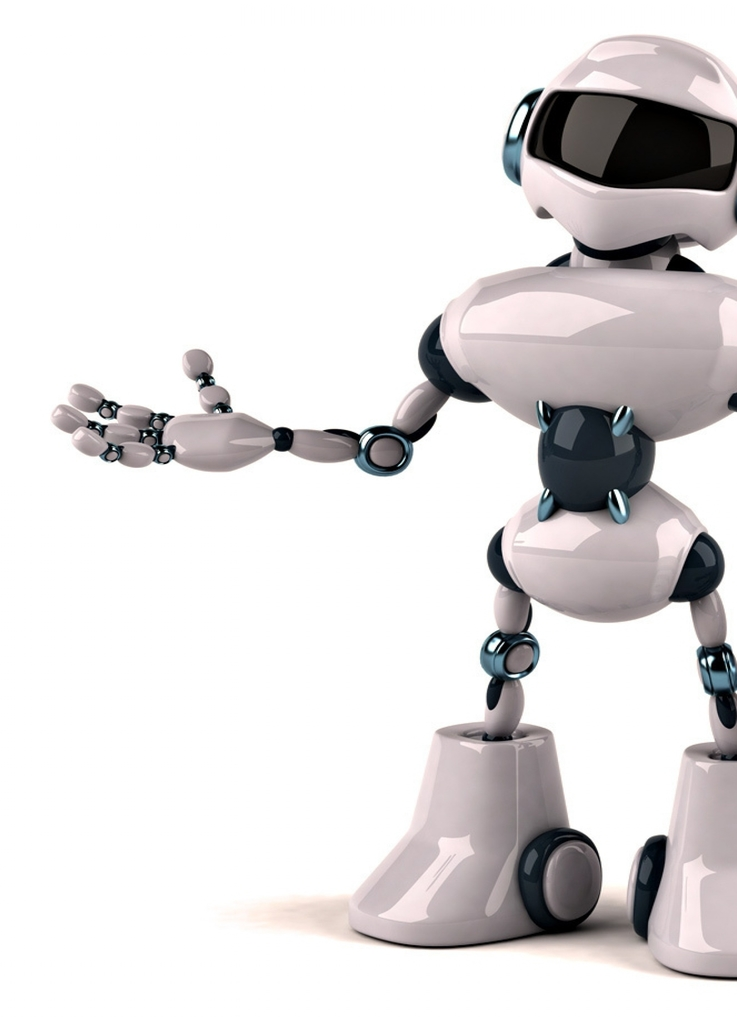
\includegraphics[width=\paperwidth]{robotics-wp}}; % Background image
\draw[anchor=north] (midpoint) node [fill=ocre!30!white,fill opacity=0.6,text opacity=1,inner sep=1cm]{\Huge\centering\bfseries\sffamily\parbox[c][][t]{\paperwidth}{\centering 실전 ROS 시스템 구축\\[30pt] % Book title
{\Large Python, Matlab을 이용한 ROS}\\[20pt] % Subtitle
{\huge Donghoon Park}}}; % Author name
\end{tikzpicture}};
\end{tikzpicture}
\vfill
\endgroup

%----------------------------------------------------------------------------------------
%	COPYRIGHT PAGE
%----------------------------------------------------------------------------------------

\newpage
~\vfill
\thispagestyle{empty}

\noindent Copyright \copyright\ 2016 Donghoon Park\\ % Copyright notice

\noindent \textsc{Published by Publisher}\\ % Publisher

\noindent \textsc{sigma.snu.ac.kr}\\ % URL

\noindent GPL License

\noindent \textit{First printing, June 2016} % Printing/edition date

%----------------------------------------------------------------------------------------
%	TABLE OF CONTENTS
%----------------------------------------------------------------------------------------

%\usechapterimagefalse % If you don't want to include a chapter image, use this to toggle images off - it can be enabled later with \usechapterimagetrue

\chapterimage{chapter_head_1.pdf} % Table of contents heading image

\pagestyle{empty} % No headers

\tableofcontents % Print the table of contents itself

\cleardoublepage % Forces the first chapter to start on an odd page so it's on the right

\pagestyle{fancy} % Print headers again

%----------------------------------------------------------------------------------------
%	PART
%----------------------------------------------------------------------------------------

\part{Part1}

%----------------------------------------------------------------------------------------
%	CHAPTER 1
%----------------------------------------------------------------------------------------

\chapterimage{ros-names.png} % Chapter heading image

\chapter{ROS 개요 및 환경설정}

\section{ROS란 무엇인가}\index{Paragraphs of Text}


ROS는 Robot Operating System 으로, 로봇과 관련된 여러 패키지를 제공하고,
특히 프로시저간의 안전한 통신 규약을 제공하는 프로그램입니다.
Operating System이라는 이름 때문에 오히려 ROS의 개념에 대해 헷갈려하는 분들이 계신데,
ROS는 OS가 하는 일을 일부 도맡아서 하는 프로그램으로 생각하시면 됩니다.

ROS는 2016년 6월 시점으로 ROS Kinetic 버전까지 나와있으며, ROS의 마스코트는 왜인지 모르겠지만 거북이이고,
레퍼런스 로봇은 꼬부기(turtlebot)이고, 예제도 거북이로 시작합니다. ROS는 설치하는 과정 자체가 기존 Linux유저 기준으로 어려운 편은 아니지만,
로봇을 만드는 사람들이 모두 Linux에 익숙한 것은 아니기 때문에 설치 난이도가 낮은 편은 아닙니다.
어떻게 보면 매우 어려운 설치 과정을 거치는데, 이런 고생을 하면서까지 왜 ROS를 사용해야 하는지에 대해 이야기해보도록 하죠.


\includegraphics[scale=0.3]{ros-kinetic}

ROS의 필요성에 대해 이야기하려면 ROS가 어떤 것인지부터 이야기해야 할 것입니다.
프로그래머의 입장에서 보면, ROS는 일종의 라이브러리입니다. Python, C++, Matlab, Javascript 등에서 돌아가는 라이브러리를 공식적/ 비공식적으로 제공하며,
프로그램 언어에서 쉽게 불러와서 사용할 수 있습니다. ROS 라이브러리가 제공하는 API는 상당히 단순합니다.
데이터를 저장하고 불러오는 두 가지 방식에 대한 함수(or Functional Block)를 제공할 뿐입니다.
여기서 의문이 들 수 있습니다.리눅스에 조금 익숙하신 분이라면 알겠지만 리눅스에서는 변수 공유를 그다지 어려운 과정을 거치지 않고 할 수 있습니다.
왜 굳이 ROS를 써야 하는것일까요? 그 해답은 ROS의 호환성에 있다고 할 수 있습니다. ROS는 다른 언어간에도 심지어 다른 하드웨어간에도 변수 공유를 위한 프로토콜을 제공합니다.
그리고 무엇보다도 프로그램을 패키지화 시키고 나면, 우리가 프로그램의 내부를 아얘 모르고도 그 패키지에서 뽑아주는 변수만 사용할 수 있다는 점이 가장 큰 장점이죠.
사실상의 하드웨어 플러그 앤 플레이를 진정하게 가능하게 하는 것이죠.
ROS 패키지를 이용할 때는 소프트웨어 패키지는 설치 후 실행만 하면 됩니다. 하드웨어 연결이 필요한 패키지는 동일한 하드웨어 구성 후 꽂고, 패키지를 실행하면 됩니다.
기존에 개발한 하드웨어에 대한 완벽한 재사용성을 확보할 수 있는 것이죠.
임베디드 환경에서 구르던 로봇 프로그래머들에게 조금 더 감을 잡을 수 있게 예시를 들어보자면,
다른 사람이 짠 아두이노 시스템을 컴퓨터에 꽂기만 하면 주요 변수를 ROS가 directory 형식으로 정리해서 보여준다는 말도 안되는 일이 가능해집니다.

결론적으로, 하드웨어 및 소프트웨어의 모듈화 및 재사용성을 극한까지 추구할 수 있는 구조가 ROS라고 보시면 됩니다.


%------------------------------------------------

\section{ROS를 사용하기 위해서는?}\index{ROS를 사용하기 위해서는?}

ROS를 사용하기 위해서는 먼저 시스템을 구성해야 합니다. ROS는 보통 Ubuntu라는 리눅스 배포판 위에
올려서 쓰는 것이 일반적입니다. Ubuntu 위에서는 ROS를 비교적 쉽게 명령줄 도구를 이용해서 설치할 수 있습니다.
또한, Ubuntu는 리눅스 배포판 중 매우 유명한 축에 속하며 ARM 보드를 상당히 잘 지원하기 때문에 소형 로봇 시스템에도 올릴 수 있다는 점에서 Ubutu 위에서 ROS 구성 후 실습을 하시는 것을 권장합니다.

그리고, ROS에 접속하는 프로그램을 짜는 과정 또한 필요하기 때문에 개발용 프로그램 언어 환경 또한 설치해야 합니다.
보통 ROS 접속 프로그램을 짤 떄는 Python, C++ 등의 언어를 사용합니다. 이 책에서는 Python을 주 개발 언어로 사용하는 과정에 대해 이야기하겠습니다.
보다 나은 성능을 원한다면 C++을 이용하는 것을 권장합니다. ros 기본 메뉴얼은 C++로 작성되어있기 때문에, 기본 ros 매뉴얼을 따라서 한다면 C++ 프로그래밍은 어렵지 않게 할 수 있습니다.
이 교재에서 Python을 주 언어로 사용하는 이유는 스크립트 인터프리터를 이용한 실시간 코드 확인이 가능하기 때문입니다. 다시 한번 강조하지만 프로그램이 무거운 경우 C++에서의 개발을 권장합니다.

또한 이것은 필자의 개인적인 추천인데, Matlab을 활용할 수 있는 환경에 있고, 로봇의 Computing Power가 충분히 좋은 경우 Matlab의 Simulink를 사용하는 것을 추천합니다.
Matlab Simulink는 Gui Block Programming Language로 시스템 구성에 있어서는 매우 탁월한 기능을 갖추고 있습니다.
특히, DSP Filter 구성에서는 따라올 대안이 없다는 것에는 대부분의 엔지니어가 동의할 것입니다.

따라서 본 교재를 전부 보기 위해서는 아래와 같은 환경을 구성하고 가는 것을 추천합니다.

\begin{enumerate}
\item Ubuntu 14.04 or Ubuntu 16.04
\item ROS Jade or Kinetic
\item Python 2.7 and Development Environment
\item Matlab 2016a with Simulink Robotics Communication Block
\item Arduino or Mbed
\end{enumerate}

이제 Arduino를 제외한 (아두이노는 인간적으로 너무 쉬워요..) 해당 환경들을 설치하는 방법에 대해서 차근차근 설명해 보겠습니다.

%------------------------------------------------

%------------------------------------------------
\section{Ubuntu 설치}
\label{sec:Ubuntu 설치}

이번 섹션에서는 Ubuntu를 설치하는 방법에 대해 이야기해 보겠습니다. Ubuntu는 앞서 말했듯이 리눅스 시스템으로,
ROS를 올리기 좋은 환경을 제공해줍니다. 하드웨어를 연계해서 개발을 할 예정이니 Virtual Machine이 아닌 Native로 설치하는 것을 권장합니다.
ARM 보드 위에 설치한 Ubuntu를 가지고 교재를 진행하는 것은 권장하지 않습니다. 왜냐하면 ARM에는 지원되지 않는 ROS 패키지가 많으며, 이 교재는 64비트 x86 CPU (일반적인 Intel, AMD CPU) 기준으로 쓰여졌기 때문입니다.

먼저 Ubuntu ISO Image를 다운로드 받습니다. 우분투 공식 배포판을 활용하는 것을 추천합니다.

\begin{link}[http://www.ubuntu.com/]
  : Ubuntu 공식 홈페이지
\end{link}

 Ubuntu 공식 홈페이지에 접속하셔서 Desktop 버전을 다운로드 받으세요. LTS(Long Term Support) 버전을 사용하는 것을 추천합니다.


\begin{figure}[h]
\centering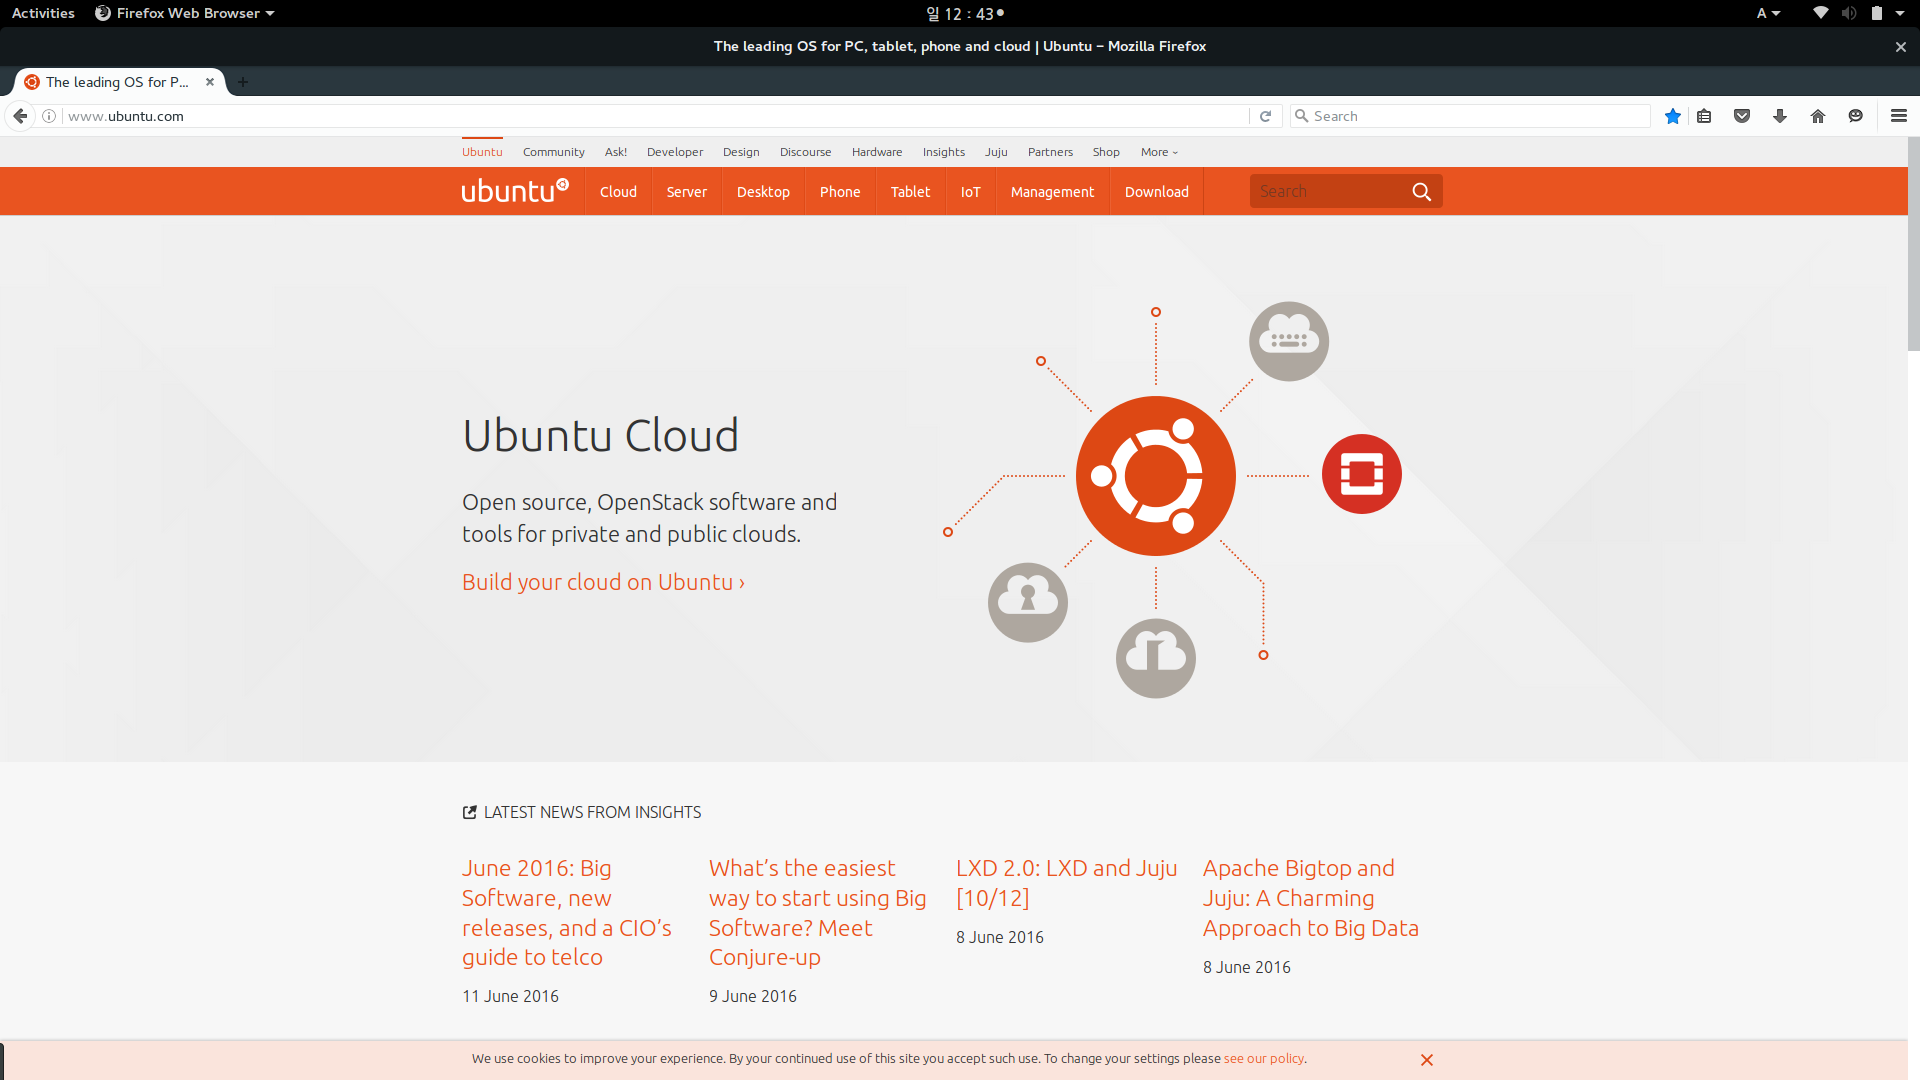
\includegraphics[scale=0.22]{01_ubuntu_mainpage}
\caption{Ubuntu 공식 페이지}
\end{figure}

다운로드 받은 ISO 파일은 이제 usb에 넣어 부팅 usb를 만들고 설치해야 합니다.
해당 과정은 잘 정리되어 있는 블로그 링크가 있기에 아래에 첨부합니다.

\begin{link}[http://sergeswin.com/1178]
: Ubuntu 부팅 usb 제작과정
\end{link}

해당 블로그의 글을 보고 부팅 usb를 만드셨다면, 이제 컴퓨터 파티션에 공간을 30GB정도 남긴 뒤(단순히 free space가 아니라 disk 관리로 들어가셔서 가용 공간을 확보하셔야 합니다.) usb로 부팅해서 해당 공간에 ubuntu를 설치하세요.
공식 홈페이지에서 튜토리얼을 제공하니 참고하셔서 설치하면 어렵지 않게 설치가 가능합니다.

\begin{link}[http://www.ubuntu.com/download/desktop/install-ubuntu-desktop]
: Ubuntu 설치 과정
\end{link}

사실 Ubuntu는 리눅스 중에서도 매우 사용자 친화적인 배포판이기 때문에 설치순서 자체가 어렵다기보다는, 설치 과정 중에 생기는 문제가 해결하기 까다롭습니다.
그러나 개인별 증상이 매우 다르고, 그 때마다 해결책도 다르기 때문에 모든 것을 매뉴얼로 만들기는 사실상 불가능합니다.
Ubuntu 설치 중에 문제가 생긴다면 아래 사이트를 참고해서 해결하도록 노력해보세요.
Linux 환경에서 작업읋 하기 위해서는 해당 배포판의 포럼을 계속해서 들락 날락 하는 노력이 필요하답니다.

\begin{link}[http://askubuntu.com/]
: AskUbuntu Forum
\end{link}

무사히 Ubuntu를 설치하셨다면 축하합니다! 다음 파트에서는 드디어 ROS를 설치해 보겠습니다.

%------------------------------------------------

\section{ROS 설치}\index{ROS 설치}

ROS는 2016.06 현재 ROS Kinetic Version 까지 나와 있습니다. ROS 또한 Ubuntu와 마찬가지로 여러 가지 배포판이 나와있는데, 일반적으로 비슷한 시기에 나온 Ubuntu와 ROS 배포판이 호환성이 좋습니다.
Ubuntu 14.04를 설치해 온 분은 ROS Jade, Ubuntu 16.04를 설치해 온 분은 ROS Kinetic을 권장합니다. 혹시나 개발기간이 촉박해서 기존 패키지를 조합하는 방식의 개발을 원하는 분은 구버전인 ROS Indigo를 사용하셔도 좋습니다.
ROS는 최신버전으로 올수록 apt-get을 이용해 간단히 설치할 수 있는 패키지가 줄어들기 때문에, 최신버전과 패키지의 숫자 사이에서 잘 저울질 해서 알맞은 버전을 선택하시길 바랍니다.

\begin{figure}[h]

\includegraphics[scale=2.0]{02_ros_indigo}
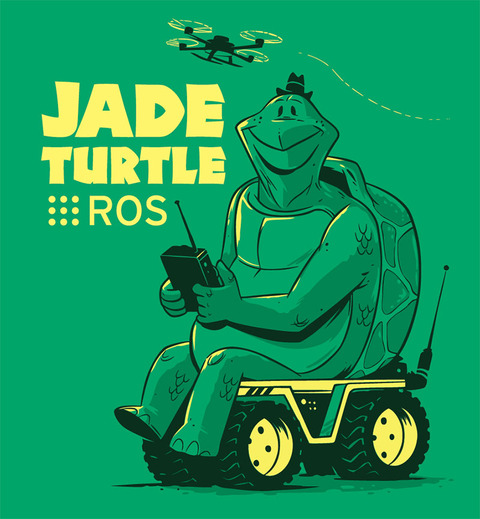
\includegraphics[scale=0.3]{03_ros_jade}

\includegraphics[scale=0.2]{04_ros_kinetic}
\caption{ROS Versions}
\end{figure}

ROS 설치를 위해서는 Ubuntu에서 커멘드 라인을 실행해야 합니다.
일반적인 환경을 구축했다면 Ctrl + Alt + T 를 누르면 아래와 같이 커멘드라인이 실행됩니다.

\begin{figure}[h]
\centering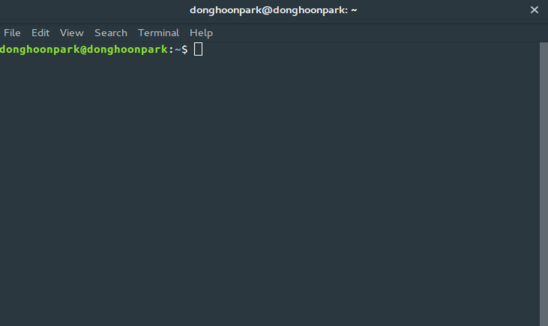
\includegraphics[scale=0.7]{05_terminal}
\caption{Terminal 실행 창}
\end{figure}

이제 이 창 위에 설치 명령어를 입력하여 ROS를 설치하게 됩니다. ROS설치는 대부분 비슷한 과정으로 진행되지만, 버전별로 약간씩 상이하기 때문에
자신이 설치할 버전이 무엇인지 잘 알고 진행하시기 바랍니다. 혹시나 ARM Linux Board(Odroid/ Raspberry pi/ Beaglebone Black)가
최종 Target System인 경우, 최신버전인 ROS Kinetic을 설치하지 않는 것을 권장합니다.

ROS의 버전별 설치 방법은 아래와 같습니다.

\begin{link}[http://wiki.ros.org/indigo/Installation/Ubuntu]
  : ROS Indigo 설치과정
\end{link}

\begin{link}[http://wiki.ros.org/jade/Installation/Ubuntu]
  : ROS Jade 설치과정
\end{link}

\begin{link}[http://wiki.ros.org/kinetic/Installation/Ubuntu]
  : ROS Kinetic 설치과정
\end{link}

설치 과정에 따라 명령어를 입력하면 ROS가 설치됩니다. desktop-full package로 설치하는 것을 권장드리며,
최대 약 1시간까지도 걸리는 작업이므로 느긋하게 기다려 주세요.
1.1 - 1.8 까지 모든 명령어를 순서대로 입력하셔야 합니다.

간단하게 설치하고 싶으시다 혹은 리눅스 초보라 아무것도 모르겠다 하시는 분은 아래 명령어를 입력해서 ROS Indigo를 간단하게 설치하는 방법도 있습니다만 권장하지 않습니다.
해당 링크는 오픈소스 로보틱스 카페 표윤석 연구원님꼐서 만든 저장소와 스크립트입니다.

\begin{link}[http://cafe.naver.com/openrt/13991]
  : wget https://raw.githubusercontent.com/oroca/oroca-ros-pkg/master/ros\_install.sh\, \&\& chmod 755\, ./ros\_install.sh\, \&\& ./ros\_install.sh\, catkin\_ws indigo
\end{link}

ROS를 모두 설치했다면 제대로 설치되었는지 roscore 프로그램을 실행시켜 봅시다.
터미널을 열고, roscore 명령어를 아래와 같이 입력하고 실행해 보세요. 정상적으로 작동한다면 ROS 설치에 성공한 것입니다. 아래 예시는 ROS Kinetic을 설치한 예시입니다.

\begin{figure}[h]
\centering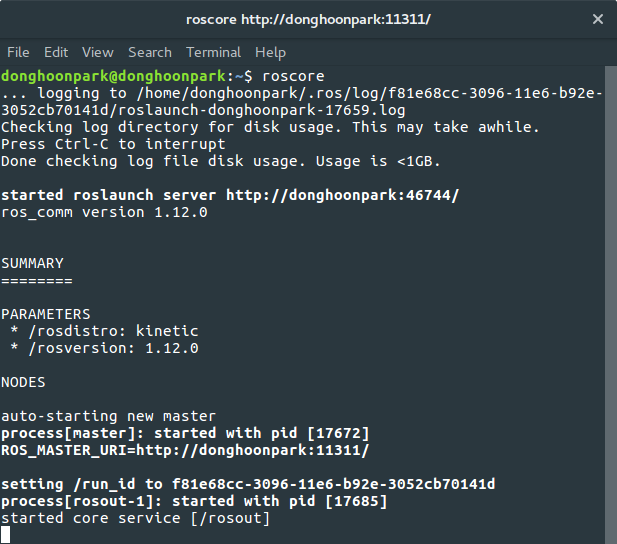
\includegraphics[scale=0.5]{06_roscore_terminal}
\caption{roscore 실행 창}
\end{figure}


%------------------------------------------------
\section{Python Development Environment}\index{Python Development Environment}

이제 프로그래밍 언어인 파이선을 사용하기 위한 개발환경을 갖추어 봅시다.
프로그래밍 언어 개발환경은 크게 세 가지로 구성됩니다. Editor, Compiler, Debugger.
여기에서는 IDE 한 가지를 추천하고, 혹시나 상황이 여의치 않을 경우 사용할 수 있는 오픈소스 개발환경 구축법을 소개하도록 하겠습니다.

\subsection{Pycharm}\index{Pycharm}

\begin{figure}[h]
\centering
\includegraphics[scale=0.5]{07_pycharm}
\caption{pycharm}
\end{figure}

Pycharm은 Jetbrains에서 만든 Python 전용 IDE입니다. 파이선 패키지만 설치된 상태라면 자동으로 모든 설정을 알아서 수행하며, 설치만 하면 바로 사용할 수 있는 상태가 됩니다.
아쉬운 점이라면 다른 환경에 비해 비교적 무겁다는 점과, 무료가 아니라는 점입니다. 그러나 학생인증을 하면 무료로 받을 수 있으므로 학생이라면 해당 IDE를 사용하는 것을 권장합니다.
개인적인 감상으로는 여타 개발 프로그램에 비해 비싼 편이 아니므로 구매하는 것도 상당히 좋은 선택일 것입니다.(필자는 위 회사와 아무런 관련이 없습니다.)
Pycharm은 아래 링크로 가면 다운로드 받을 수 있습니다.

\begin{link}[https://www.jetbrains.com/pycharm/]
  : Pycharm 공식 홈페이지
\end{link}

\begin{figure}[h]
\centering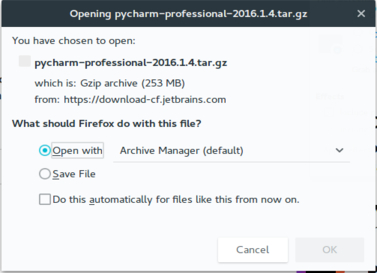
\includegraphics[scale=0.5]{08_pycharm_download}
\caption{pycharm 다운로드}
\end{figure}

Pycharm을 다운로드 받고, 설치하는 방법에 대해 이야기하겠습니다. tar.gz 확장자를 가진 파일은 tar 명령어 혹은 파일 압축풀기 프로그램을 이용해 압축을 해제할 수 있습니다.
압축을 푸는 법은 검색해서 찾아보시고, 압축이 풀린 상태에서 아래 그림과 같이 커멘드라인에서 해당 경로로 이동 후 실행파일을 실행(./) 시켜주면 됩니다.

\begin{figure}[h]
\centering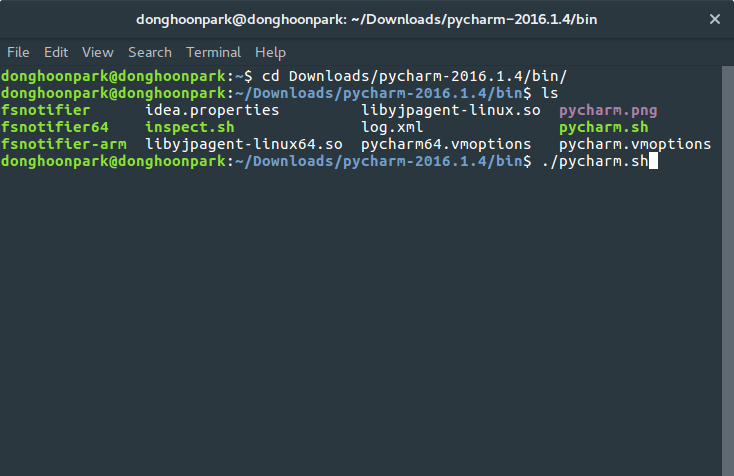
\includegraphics[scale=0.4]{09_pycharm_install}
\caption{pycharm 설치}
\end{figure}

\begin{figure}[h]
\centering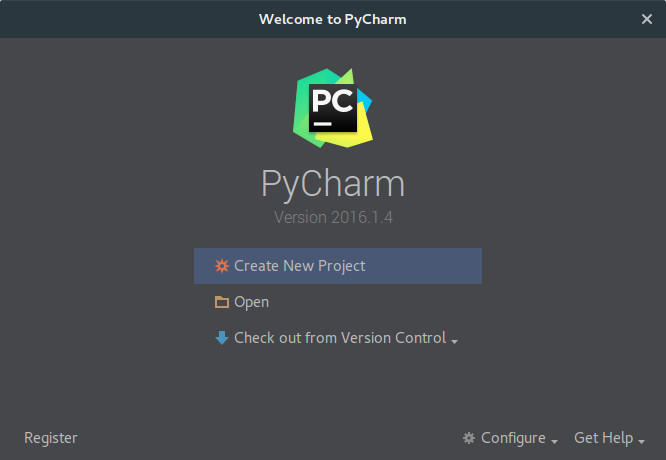
\includegraphics[scale=0.4]{10_pycharm_installed}
\caption{pycharm 실행화면}
\end{figure}

이제 new project를 누르고 프로그래밍을 시작하면 됩니다. Pycharm을 설치했다면 이후 단계를 생략해도 좋습니다.

\subsection{Python Package Install}\index{Python Package Install}

IDE를 사용하지 않는 경우에는 IDE에 해당하는 환경을 각각 구성해줘야 합니다. 각각의 환경이 또 파이선을 사용하는 경우가 많아 파이선 패키지 관리자를 먼저 설치하고 시작하도록 하겠습니다.
아래의 명령어 한 줄이면 Python Package 관리자인 pip이 설치됩니다.

\# sudo apt-get install python-pip

이제 pip에서 아래의 패키지들을 명령줄 도구로 설치해봅시다.

\# sudo pip install jedi

\# sudo pip install pylama

jedi는 파이선 언어 자동완성 패키지이고, pylama는 파이선 언어 코드 형식 및 에러체크 패키지입니다.

\subsection{Atom Editor Install}\index{Atom Editor Install}

이제 에디터를 설치하고 위에서 설치한 파이선 패키지들을 연결해봅시다.

\begin{figure}[h]
\centering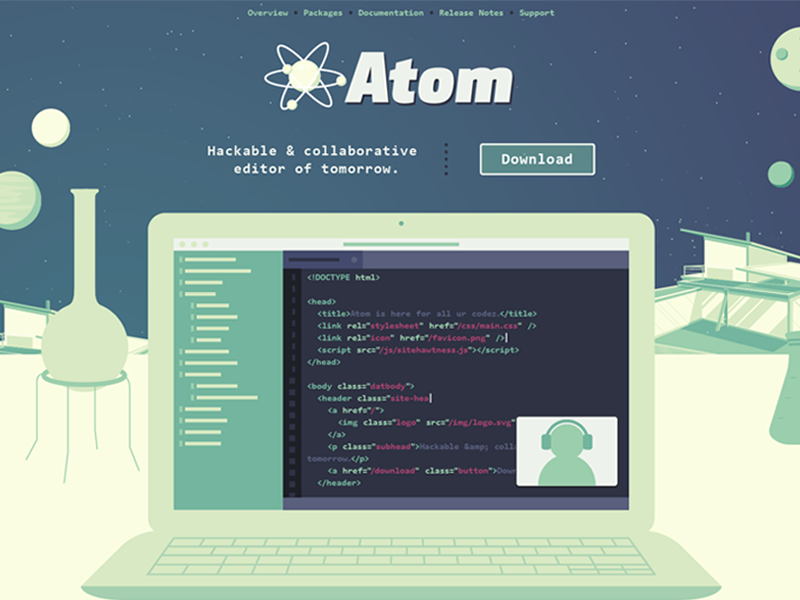
\includegraphics[scale=0.45]{11_atom}
\caption{Atom Editor}
\end{figure}

Atom은 Github에서 만든 에디터로, 상당히 사용자 친화적인 인터페이스를 제공합니다.
물론 속도가 조금 느리다는 평이 있지만, 속도를 중요시하는 분들은 Vim이나 Emacs를 알아서 잘 사용하실 것으로 믿기에 에디터는 Atom 에디터만 다루고 넘어가도록 하겠습니다.
아래 링크로 들어가서 Atom editor 패키지를 받습니다.(.deb)

\begin{link}[https://atom.io/]
  : Atom Editor 공식 홈페이지
\end{link}

.deb 패키지는 실행시키면 소프트웨어 센터에 연결되며 설치가 될 것입니다. 이제 위 파이선 패키지들에 연결할 에디터 패키지를 설치해봅시다.
atom을 실행한 후 Ctrl+, 를 누르면 세팅 메뉴가 열리고, 여기서 새로운 패키지들을 설치할 수 있습니다.

\begin{figure}[h]
\centering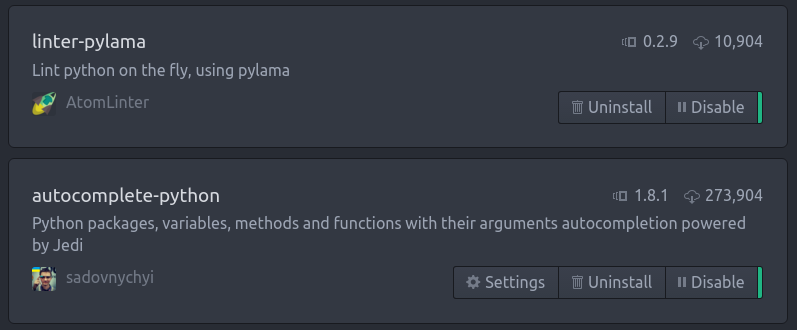
\includegraphics[scale=0.4]{12_atom_packages}
\caption{Atom Install Packages}
\end{figure}

위에 있는 두 패키지를 설치하면 됩니다. 이제 ROS를 손쉽게 사용할 수 있도록 autocomplete-python package를 설정하겠습니다.
그 전에 ROS용 파이선 패키지 설치 경로를 알아야 설정이 가능하므로 아래와 같이 Python 쉘을 실행시켜 ROS 모듈을 위치를 알아냅니다.

\begin{figure}[h]
\centering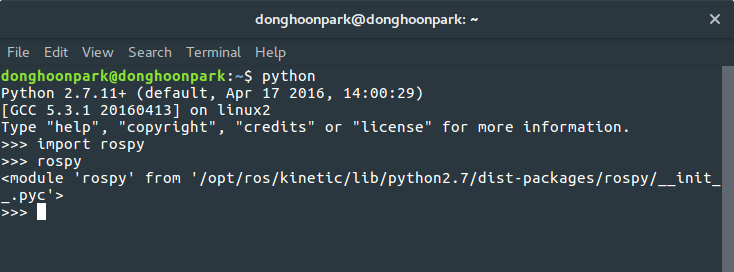
\includegraphics[scale=0.5]{13_ros_module_location}
\caption{ROS 모듈 위치 찾는법}
\end{figure}

아래 창에서 보면 rospy 모듈은 /opt/ros/kinetic/lib/python2.7/dist-packages 에 있는 것을 알 수 있습니다.
해당 경로를 복사해서 jedi 패키지 설정의 Extra Paths for Packages에 넣어줍니다. 그리고 에디터를 재시작한 후 python 파일을 하나 만듭니다.
정상적으로 설치된 경우 아래와 같이 autocompletion과 linter가 잘 작동합니다.

\begin{figure}[h]
\centering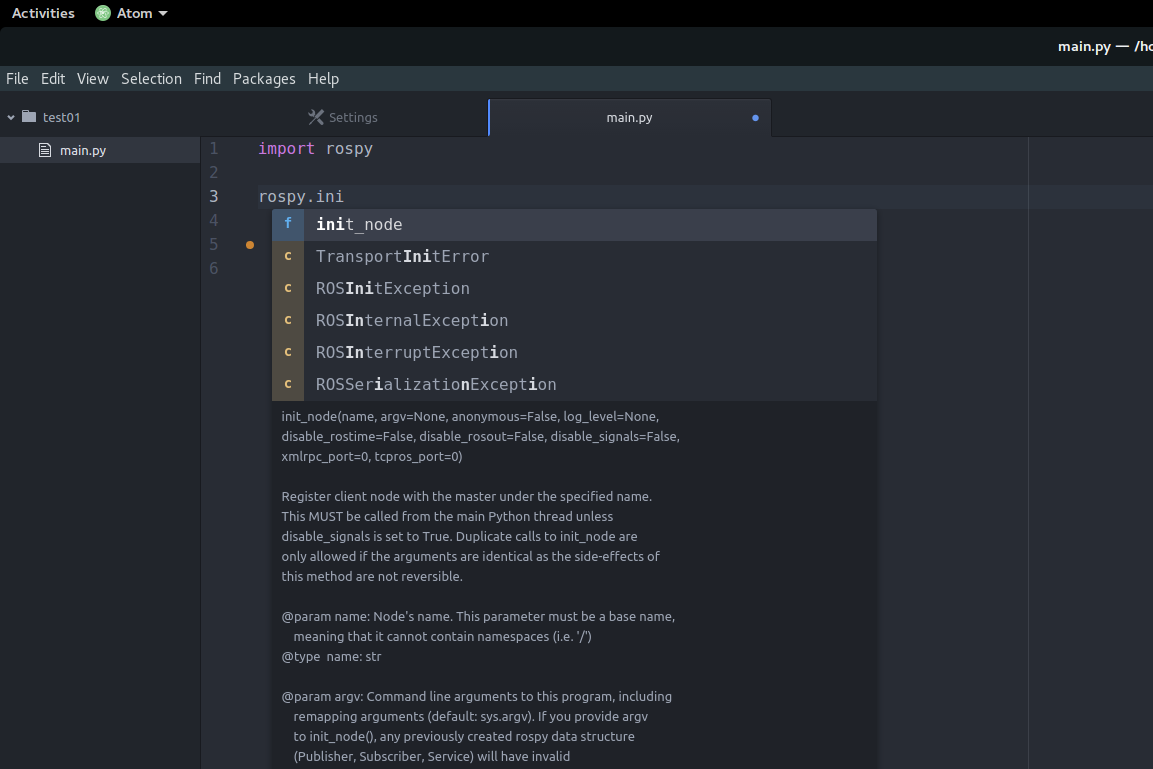
\includegraphics[scale=0.35]{14_atom_setup_complete}
\caption{Atom 정상 실행 상황}
\end{figure}

파이선 개발용 패키지들은 이것 이외에도 유용한 것이 많으니 개인의 취향에 따라 선택해서 더 많은 패키지를 이용해 생산성을 높여보시기 바랍니다.


\section{Matlab Install}\index{Matlab Install}

마지막으로 Matlab을 설치합니다. (학교 혹은 기관 라이선스가 있는 경우에)

\begin{figure}[h]
\centering
\includegraphics[scale=0.7]{15_matlab}
\caption{Matlab}
\end{figure}

Matlab 설치 과정은 Mathworks 사에 매우 자세하게 설명되어있기 때문에 생략하도록 하겠습니다.
ROS 지원 블록을 설치하는 것을 잊지 마세요. 아래 링크를 이용해서 접속하시면 Matlab을 받을 수 있습니다.

\begin{link}[http://kr.mathworks.com/downloads/web\_downloads/?s\_tid=srchtitle   ]
  : Matlab 다운로드 페이지
\end{link}

설치가 완료되면 아래 한 줄 커멘드 라인으로 Matlab 우분투 지원 패키지를 설치하세요. Matlab을 시스템에 알맞게 Integration 시켜주고, 명령줄 상에서 Matlab을 실행할 수 있게 해주는 도구입니다.

\#sudo apt-get install matlab-support

아래와 같이 커맨드라인에서 Matlab을 실행해보는 것으로 Chapter1을 마치겠습니다.

\begin{figure}[h]
\centering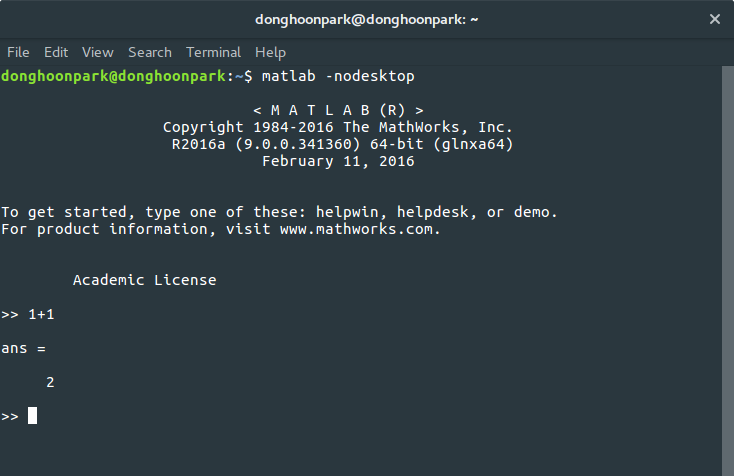
\includegraphics[scale=0.4]{16_matlab_test}
\caption{Matlab Command Line Test}
\end{figure}

%------------------------------------------------

% \section{Citation}\index{Citation}
%
% This statement requires citation \cite{book_key}; this one is more specific \cite[122]{article_key}.
%
% %------------------------------------------------
%
% \section{Lists}\index{Lists}
%
% Lists are useful to present information in a concise and/or ordered way\footnote{Footnote example...}.
%
% \subsection{Numbered List}\index{Lists!Numbered List}
%
% \begin{enumerate}
% \item The first item
% \item The second item
% \item The third item
% \end{enumerate}
%
% \subsection{Bullet Points}\index{Lists!Bullet Points}
%
% \begin{itemize}
% \item The first item
% \item The second item
% \item The third item
% \end{itemize}
%
% \subsection{Descriptions and Definitions}\index{Lists!Descriptions and Definitions}
%
% \begin{description}
% \item[Name] Description
% \item[Word] Definition
% \item[Comment] Elaboration
% \end{description}

%----------------------------------------------------------------------------------------
%	CHAPTER 2
%----------------------------------------------------------------------------------------

\chapter{ROS Basics}

\section{ROS Topic}\index{ROS Topic}

ROS에서 Topic은 비동기로 작동하는 시스템 변수로 볼 수 있습니다. 이 변수를 발행하는 곳(일반적으로 센서)을 Publisher라고 부르고,
이 변수를 받아들이는 곳 (일반적으로 Actuator 등)을 Subscriber라 부르죠. 두 가지 기능을 동시에 하는 경우 (Filter)도 존재할 수 있습니다.
ROS 내용에 대한 보다 개념적인 자세한 설명은 아래 링크의 표윤석 수석연구원님의 책 53p-67p를 참고하기 바랍니다.

\begin{link}[https://github.com/robotpilot/rosbook\_kr/blob/master/pdf/ROS\_Book\_KR.pdf]
  : 로봇 프로그래밍 ROS로 시작하자! - 표윤석 수석연구원님 저
\end{link}

간단한 Line Follower Robot을 ROS로 구성한다고 했을 때 아래 그림과 같이 시스템을 구성해볼 수 있습니다.

\begin{figure}[h]
\centering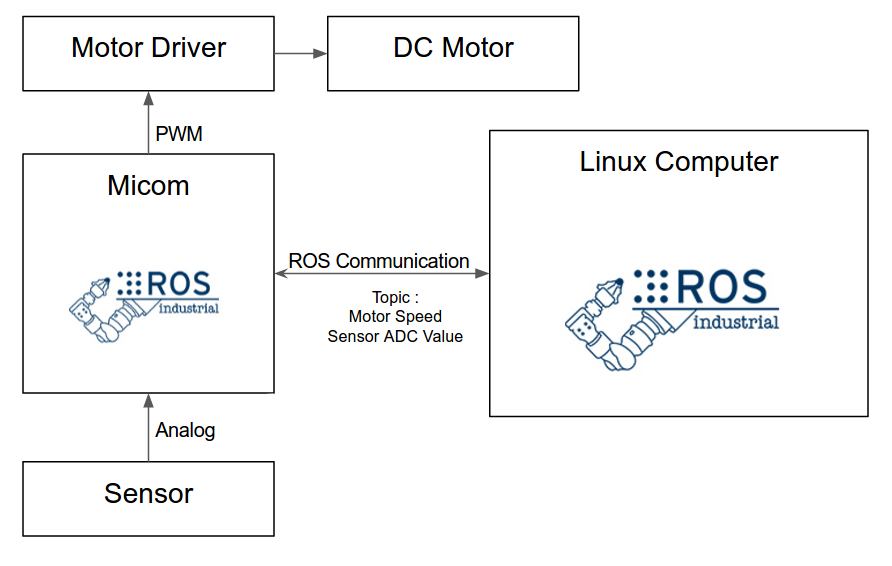
\includegraphics[scale=0.3]{17_ros_system_example}
\caption{ROS System example}
\end{figure}

센서 데이터는 Micom(Arduino, Mbed, STM32 등등)에서 일차적으로 ADC로 읽어오게 됩니다. 그리고 ADC로 읽은 데이터를 ROS에 Publish 하면 ROS 입장에서는 Data가 일정 주기로 계속 업데이트 되는 것으로 보이죠.
모터를 제어할 때도 마찬가지입니다. ROS에서 모터 출력에 대한 변수를 하나 Publish하고, 실제로 모터를 제어하는 Micom이 해당 데이터를 Subscribe하면서 업데이트하면 ROS에서 모터제어를 할 수 있습니다.

\section{Topic Publisher}

\subsection{Rqt를 이용한 Topic Publisher}

시뮬레이션 프로그램을 매우 간단하게 구동해 보면서 Topic을 Publish 한다는 것이 어떤 의미인지 감을 잡아봅시다. ROS는 시뮬레이션 모델에 대한 정보를 Topic으로 불러올 수 있습니다.
해당 Topic들은 시뮬레이션 모델의 물리 벡터를 가지고 있습니다.(Torque, Force 등)
이것들을 Control 하는 방법으로 시뮬레이션을 구동시킬 수 있죠. Topic이 어떤 형태로 나오는지 알아보기 위해서 Gazebo Robot Simulator를 구동해봅시다.
아래의 명령어를 입력하면 Gazebo를 ros에 연결된 상태로 구동할 수 있습니다.

\#rosrun gazebo\_ros gazebo

정상적으로 실행되면 아래와 같은 창을 보실 수 있습니다. 여기에서 컨트롤 할 대상인 Sphere를 하나 불러와 봅시다.

\begin{figure}[h]
\centering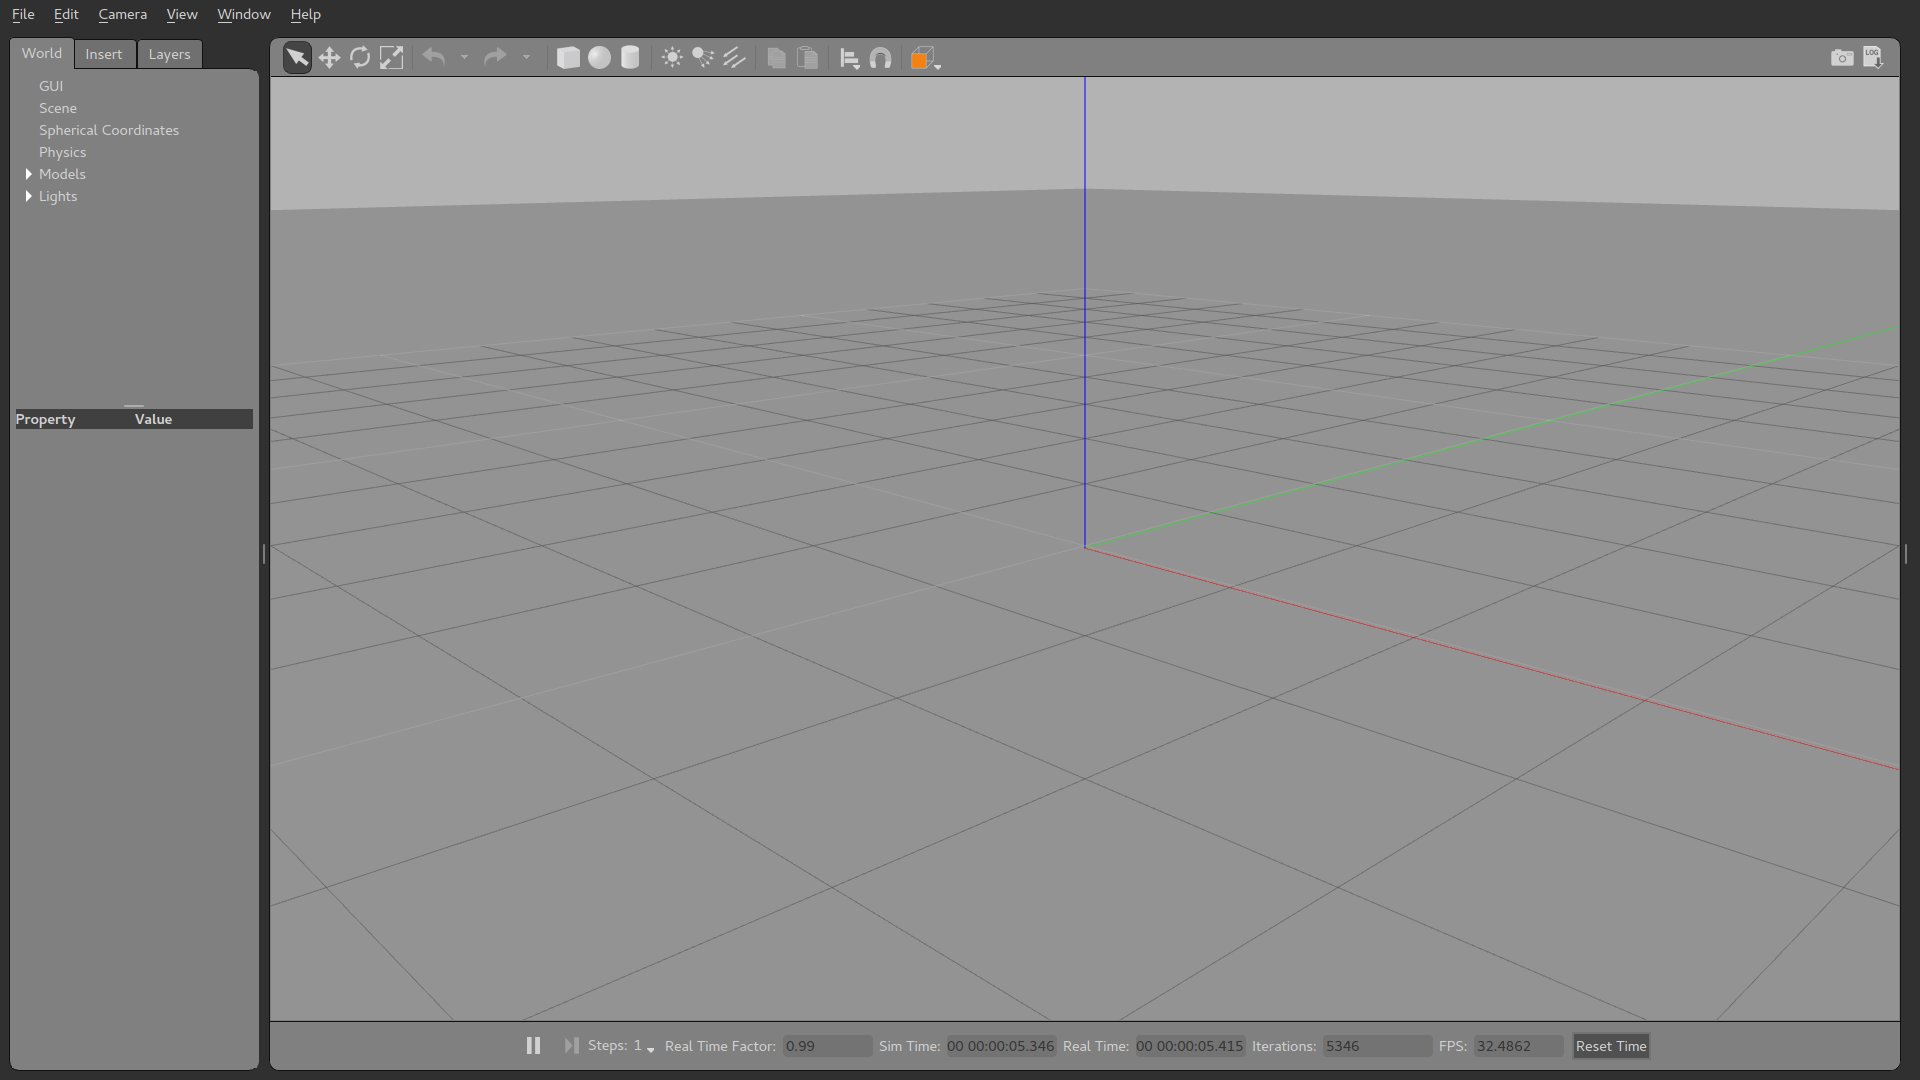
\includegraphics[scale=0.2]{18_gazebo_launch}
\caption{Gazebo 기본 화면}
\end{figure}

gazebo가 정상적으로 구동된 뒤에는 다른 터미널에서 rqt를 구동해봅니다.
rqt에서는 기본 topic publisher를 제공합니다. Plugins -> Topics -> Message Publisher를 열어보세요.

\begin{figure}[h]
\centering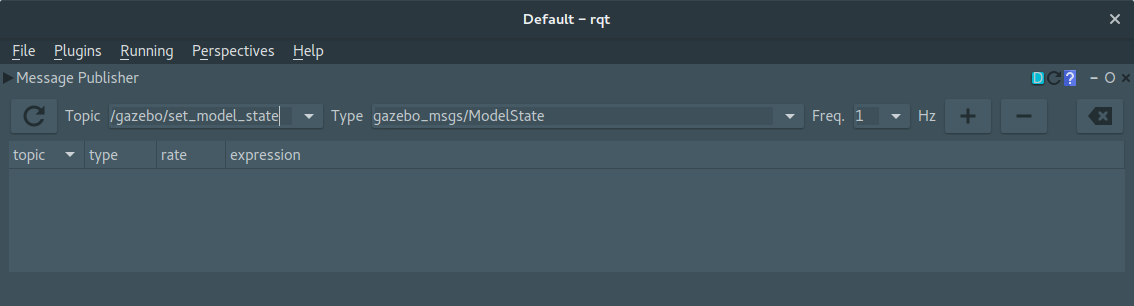
\includegraphics[scale=0.35]{19_rqt_gazebo_topic}
\caption{rqt topic message publisher}
\end{figure}

\#rqt

여기에서 /gazebo/set\_model\_state 라는 topic을 불러와 봅시다. 해당 topic은 Gazebo에서 Subscribe하고 있는 topic으로 해당 내용이 바뀌면
Gazebo는 프로그램에서 해당 모델의 상태를 바꾸어줍니다. 해당 topic을 publish하기 위해서 오른쪽의 \+ 버튼을 눌러 publisher를 추가합니다.
그리고 publish할 message를 아래와 같이 설정합니다. 아래와 같이 설정했을 때 i는 rate가 하나 지날 때 마다 1씩 올라가는 변수이므로, 약 63초마다 원은 원점을 따라서 한 바퀴씩 움직이게 될 것입니다.

rqt는 topic 제어 이외에도 여러 기능을 가지고 있기 때문에 간단히 훑어보시는 것도 좋을 것입니다.
특히, Matlab을 사용하지 않는 경우 rqt의 plot 기능은 매우 유용하게 사용할 수 있습니다.

\subsection{Python을 이용한 Topic }


% This is an example of theorems.
%
% \subsection{Several equations}\index{Theorems!Several Equations}
% This is a theorem consisting of several equations.
%
% \begin{theorem}[Name of the theorem]
% In $E=\mathbb{R}^n$ all norms are equivalent. It has the properties:
% \begin{align}
% & \big| ||\mathbf{x}|| - ||\mathbf{y}|| \big|\leq || \mathbf{x}- \mathbf{y}||\\
% &  ||\sum_{i=1}^n\mathbf{x}_i||\leq \sum_{i=1}^n||\mathbf{x}_i||\quad\text{where $n$ is a finite integer}
% \end{align}
% \end{theorem}
%
% \subsection{Single Line}\index{Theorems!Single Line}
% This is a theorem consisting of just one line.
%
% \begin{theorem}
% A set $\mathcal{D}(G)$ in dense in $L^2(G)$, $|\cdot|_0$.
% \end{theorem}

%------------------------------------------------
%
% \section{Definitions}\index{Definitions}
%
% This is an example of a definition. A definition could be mathematical or it could define a concept.
%
% \begin{definition}[Definition name]
% Given a vector space $E$, a norm on $E$ is an application, denoted $||\cdot||$, $E$ in $\mathbb{R}^+=[0,+\infty[$ such that:
% \begin{align}
% & ||\mathbf{x}||=0\ \Rightarrow\ \mathbf{x}=\mathbf{0}\\
% & ||\lambda \mathbf{x}||=|\lambda|\cdot ||\mathbf{x}||\\
% & ||\mathbf{x}+\mathbf{y}||\leq ||\mathbf{x}||+||\mathbf{y}||
% \end{align}
% \end{definition}
%
% %------------------------------------------------
%
% \section{Notations}\index{Notations}
%
% \begin{notation}
% Given an open subset $G$ of $\mathbb{R}^n$, the set of functions $\varphi$ are:
% \begin{enumerate}
% \item Bounded support $G$;
% \item Infinitely differentiable;
% \end{enumerate}
% a vector space is denoted by $\mathcal{D}(G)$.
% \end{notation}
%
% %------------------------------------------------
%
% \section{Remarks}\index{Remarks}
%
% This is an example of a remark.
%
% \begin{remark}
% The concepts presented here are now in conventional employment in mathematics. Vector spaces are taken over the field $\mathbb{K}=\mathbb{R}$, however, established properties are easily extended to $\mathbb{K}=\mathbb{C}$.
% \end{remark}
%
% %------------------------------------------------
%
% \section{Corollaries}\index{Corollaries}
%
% This is an example of a corollary.
%
% \begin{corollary}[Corollary name]
% The concepts presented here are now in conventional employment in mathematics. Vector spaces are taken over the field $\mathbb{K}=\mathbb{R}$, however, established properties are easily extended to $\mathbb{K}=\mathbb{C}$.
% \end{corollary}
%
% %------------------------------------------------
%
% \section{Propositions}\index{Propositions}
%
% This is an example of propositions.
%
% \subsection{Several equations}\index{Propositions!Several Equations}
%
% \begin{proposition}[Proposition name]
% It has the properties:
% \begin{align}
% & \big| ||\mathbf{x}|| - ||\mathbf{y}|| \big|\leq || \mathbf{x}- \mathbf{y}||\\
% &  ||\sum_{i=1}^n\mathbf{x}_i||\leq \sum_{i=1}^n||\mathbf{x}_i||\quad\text{where $n$ is a finite integer}
% \end{align}
% \end{proposition}
%
% \subsection{Single Line}\index{Propositions!Single Line}
%
% \begin{proposition}
% Let $f,g\in L^2(G)$; if $\forall \varphi\in\mathcal{D}(G)$, $(f,\varphi)_0=(g,\varphi)_0$ then $f = g$.
% \end{proposition}
%
% %------------------------------------------------
%
% \section{Examples}\index{Examples}
%
% This is an example of examples.
%
% \subsection{Equation and Text}\index{Examples!Equation and Text}
%
% \begin{example}
% Let $G=\{x\in\mathbb{R}^2:|x|<3\}$ and denoted by: $x^0=(1,1)$; consider the function:
% \begin{equation}
% f(x)=\left\{\begin{aligned} & \mathrm{e}^{|x|} & & \text{si $|x-x^0|\leq 1/2$}\\
% & 0 & & \text{si $|x-x^0|> 1/2$}\end{aligned}\right.
% \end{equation}
% The function $f$ has bounded support, we can take $A=\{x\in\mathbb{R}^2:|x-x^0|\leq 1/2+\epsilon\}$ for all $\epsilon\in\intoo{0}{5/2-\sqrt{2}}$.
% \end{example}
%
% \subsection{Paragraph of Text}\index{Examples!Paragraph of Text}
%
% \begin{example}[Example name]
% \lipsum[2]
% \end{example}
%
% %------------------------------------------------
%
% \section{Exercises}\index{Exercises}
%
% This is an example of an exercise.
%
% \begin{exercise}
% This is a good place to ask a question to test learning progress or further cement ideas into students' minds.
% \end{exercise}
%
% %------------------------------------------------
%
% \section{Problems}\index{Problems}
%
% \begin{problem}
% What is the average airspeed velocity of an unladen swallow?
% \end{problem}
%
% %------------------------------------------------
%
% \section{Vocabulary}\index{Vocabulary}
%
% Define a word to improve a students' vocabulary.
%
% \begin{vocabulary}[Word]
% Definition of word.
% \end{vocabulary}
%
% %----------------------------------------------------------------------------------------
% %	PART
% %----------------------------------------------------------------------------------------
%
% \part{Part Two}
%
% %----------------------------------------------------------------------------------------
% %	CHAPTER 3
% %----------------------------------------------------------------------------------------
%
% \chapterimage{chapter_head_1.pdf} % Chapter heading image
%
% \chapter{Presenting Information}
%
% \section{Table}\index{Table}
%
% \begin{table}[h]
% \centering
% \begin{tabular}{l l l}
% \toprule
% \textbf{Treatments} & \textbf{Response 1} & \textbf{Response 2}\\
% \midrule
% Treatment 1 & 0.0003262 & 0.562 \\
% Treatment 2 & 0.0015681 & 0.910 \\
% Treatment 3 & 0.0009271 & 0.296 \\
% \bottomrule
% \end{tabular}
% \caption{Table caption}
% \end{table}
%
% %------------------------------------------------
%
% \section{Figure}\index{Figure}
%
% \begin{figure}[h]
% \centering
\includegraphics[scale=0.5]{placeholder}
% \caption{Figure caption}
% \end{figure}

%----------------------------------------------------------------------------------------
%	BIBLIOGRAPHY
%----------------------------------------------------------------------------------------

\chapter*{Bibliography}
\addcontentsline{toc}{chapter}{\textcolor{ocre}{Bibliography}}
\section*{Books}
\addcontentsline{toc}{section}{Books}
\printbibliography[heading=bibempty,type=book]
\section*{Articles}
\addcontentsline{toc}{section}{Articles}
\printbibliography[heading=bibempty,type=article]

%----------------------------------------------------------------------------------------
%	INDEX
%----------------------------------------------------------------------------------------

\cleardoublepage
\phantomsection
\setlength{\columnsep}{0.75cm}
\addcontentsline{toc}{chapter}{\textcolor{ocre}{Index}}
\printindex

%----------------------------------------------------------------------------------------

\end{document}
